\documentclass[crop,tikz,border=1px]{standalone}

\usetikzlibrary{shapes,arrows,positioning,scopes}

\begin{document}
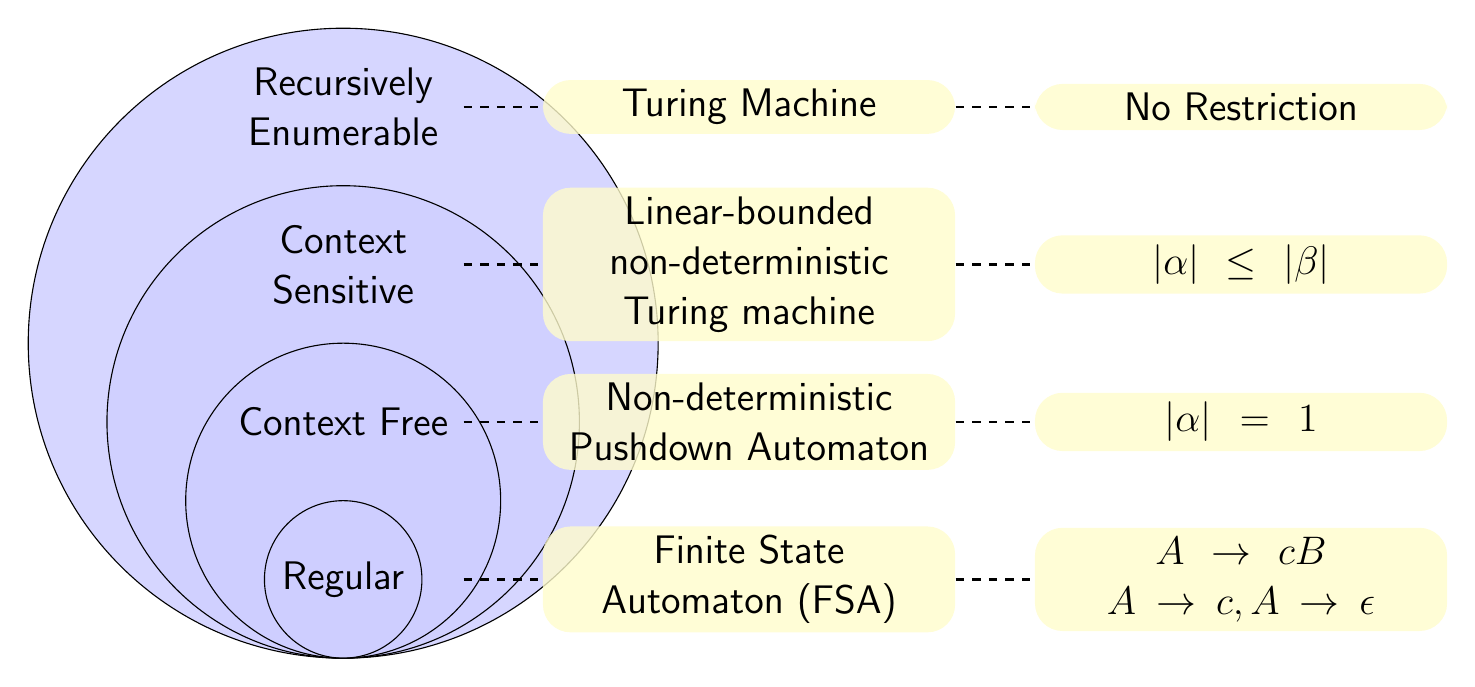
\begin{tikzpicture}[font=\Large\sffamily,
  block/.style = {fill=blue!20, minimum height=4em},
  mytext/.style = {draw=none, text centered, text width=8em, minimum height=4},
  mytext2/.style = {mytext, text width=5cm, fill=yellow!20, fill opacity=0.8, text opacity=1, rounded corners=10pt}]

  \foreach \i/\n in {4/Recursively Enumerable,3/Context
    Sensitive,2/Context Free,1/Regular}
  {
    \draw[block,fill opacity={\i * 0.2}] (0, {1 * \i}) circle (\i);
    \node[mytext] (n\i) at (0, {2 * \i - 1}) {\n};
  }

  \node[mytext2, right=1cm of n1] (t1) {Finite State\\ Automaton (FSA)};
  \node[mytext2, right=1cm of n2] (t2) {Non-deterministic\\ Pushdown Automaton};
  \node[mytext2, right=1cm of n3] (t3) {Linear-bounded\\ non-deterministic\\ Turing machine};
  \node[mytext2, right=1cm of n4] (t4) {Turing Machine};

  \node[mytext2, right=1cm of t1] (tt1) {\(A\to cB\)\\\(A\to c, A\to\epsilon\)};
  \node[mytext2, right=1cm of t2] (tt2) {\(\vert\alpha\vert = 1\)};
  \node[mytext2, right=1cm of t3] (tt3) {\(\vert\alpha\vert\leq\vert\beta\vert\)};
  \node[mytext2, right=1cm of t4] (tt4) {No Restriction};

  {[every edge/.append style={dashed, thick}]
    \foreach \i in {1,2,3,4} {
      \draw (n\i) edge (t\i)
            (t\i) edge (tt\i);
    }
  }


\end{tikzpicture}
\end{document}
